% =========================================================================== %

\begin{frame}[t,plain]
\titlepage
\end{frame}

% =========================================================================== %\\

\begin{frame}{Simultaneous}
%
\begin{columns}[T]
\column{.5\linewidth}
\vspace{-12pt}
\begin{center}
	
\includegraphics[width=.6\linewidth]{./gfx/09-xkcd-simultaneous}
\end{center}
%
\column{.5\linewidth}
\vspace{+40pt}
\begin{center}
	\emph{I'm leaving you for your twin. He's more mature than you by now.}
	
	\vspace{12pt}
	Source: \url{https://xkcd.com/514/}
\end{center}
\end{columns}
%
\end{frame}

% =========================================================================== %

\begin{frame}{Scope For Today}
%
\begin{columns}[T]
\column{.4\linewidth}
\begin{itemize}
\item Terminology in Multitasking
	\begin{itemize}
	\item Processes and Threads
	\item The GIL
	\item I/O- and CPU-bound problems
	\item Spawning and Forking
	\item Mutexes, Semaphores and Deadlocks
	\item Parallelalizability
	\end{itemize}
\item The \texttt{multiprocessing} library
	\begin{itemize}
	\item The \inPy{class Process}
	\item The \inPy{class Pool}
	\item Sharing data between processes
	\end{itemize}
\end{itemize}
%
\column{.55\linewidth}
\begin{warnbox}[Parallel Programming is hard{,} kinda]
\small
Parallel programming \emph{correctly} is notoriously difficult. The individual concepts themselves are not so hard to grasp, but they interact in unintuitive or hard to understand and control ways, and usually all of them come together at once.

\vspace{6pt}
When you want to parallelize your code, make sure it works correctly in a single thread first. Only then try to distribute the work across processors.

\vspace{6pt}
(And don't worry -- you can do it.)
\end{warnbox}
\end{columns}
%
\end{frame}

% =========================================================================== %

\begin{frame}
%
\begin{tcbraster}[raster columns=2,
                  raster equal height,
                  nobeforeafter,
                  raster column skip=0.5cm]
\begin{defbox}[Process]
\small
\begin{itemize}
\item Idea of a running program
	\begin{itemize}
	\item Several processes may act together as a single program but fundamentally independent from each other
	\item Own \emph{memory page} (\ie own variables, no way of accidentally changing another process'es memory)
	\end{itemize}
\item \emph{Scheduled} by the OS
\item Comprises of one or more \emph{threads}
\item Creation implies some overhead (\zB for allocating memory pages and for sheduling)
\end{itemize}
\end{defbox}
%
\begin{defbox}[Thread]
\small
\begin{itemize}
\item One sequence of actions belonging to a process
\item Threads in a process share memory
\item Process manages its threads
\item Fast to create, easier to (mis)handle
\item A crashed process dies alone, but a crashed thread compromises its entire host process
\end{itemize}
One program can comprise of several \emph{processes} which in turn \emph{each} can control several \emph{threads}.
\end{defbox}
\end{tcbraster}
%
\end{frame}

% =========================================================================== %

\begin{frame}
%
\begin{defbox}[The GIL (Global Interpreter Lock)]
\small
\begin{itemize}
\item System within the Python interpreter
\item Prevents multiple threads from simultaneosly accessing variables
\item[\Thus] Severely limits the use of threads in Python (see next slide)
\item[\Thus] Does not apply to using processes: Each process gets its own interpreter instance
\item[\Thus] Reasons go down deep into the guts of how Python is constructed and interacts with external libraries (\zB numpy)
\end{itemize}
\end{defbox}
%
\begin{hintbox}[Python-Implementations]
\footnotesize
There are different implementations of Python, some of which drop the GIL. You are most likely using C-Python (the most common implementation), which has a GIL. Other implemetations like PyPy or Jython buy this additional liberty at the cost of performance or interoperability with other libraries.
\end{hintbox}
%
\end{frame}

% =========================================================================== %

\begin{frame}
%
\begin{tcbraster}[raster columns=2,
                  raster equal height,
                  nobeforeafter,
                  raster column skip=0.5cm]
\begin{defbox}[CPU-Bound Problems]
\small
\begin{itemize}
\setlength{\itemsep}{0pt}
\item Botleneck is CPU
\item I.\;e. speed of computation determines runtime of program
\item Most scientific code
\item When parallelized, each parallel task needs equal access to memory
\item[\Thus] In Python: only viable with processes
\end{itemize}
\end{defbox}
%%
\begin{defbox}[I/O-Bound Problems]
\small
\begin{itemize}
\setlength{\itemsep}{0pt}
\item Bottleneck is some external device
	\begin{itemize}
	\setlength{\itemsep}{0pt}
	\item E.\;g. user input, web servers, measurement devices, ...
	\item I/O stands for input output
	\end{itemize}
\item User interfaces: maintain interoperability while doing something useful 
\item[\Thus] Threads viable (processes are, too)
\end{itemize}
\end{defbox}
\end{tcbraster}
%
\begin{hintbox}[Fuzzy Language]
\footnotesize
There is a well defined boundary between threads and processes. Still, people (me included) tend to speak about threads when meaning processes. 
This usually is not a problem, because one rarely uses both techniques in the same program. After this slide, any mention of \emph{thread} is supposed to mean \emph{process}.
\end{hintbox}
%
\end{frame}

% =========================================================================== %

\begin{frame}
%
\begin{tcbraster}[raster columns=2,
                  raster equal height,
                  nobeforeafter,
                  raster column skip=0.5cm]
\begin{defbox}[Spawning]
\small
\begin{itemize}
\item Starting a new process
\item All major operating processes support spawning
\item \enquote{Start from zero}, \ie run the first line of code
\end{itemize}
\end{defbox}
%%
\begin{defbox}[Forking]
\small
\begin{itemize}
\item Copy an existing process and continue running both
\item Unixoid OSes only (Linux, Mac, Android, etc.)
\item Continue running from wherever the fork was issued
\end{itemize}
\end{defbox}
\end{tcbraster}
%
\begin{hintbox}[Defaults and Impact]
\small
On Windows and Mac, \emph{spawn} is the default; on Linux, \emph{fork} is.

\vspace{6pt}
In practice, this difference has little impact (in Python) since we can (and should!) write code such that behaves the same whether forked or spawned. It's good to know the words though, because they tend to pop up a lot in online discussions on multitasking.
\end{hintbox}
%
\end{frame}

% =========================================================================== %

\begin{frame}{Mutexes, Semaphores and Deadlocks}
%
\begin{itemize}
\item Sometimes, a ressource shared between processes (or threads)
	\begin{itemize}
	\item E.\;g. (inter-process-) variables, screen, hard disk, ... 
	\end{itemize}
\item Possible to temporarily \emph{lock} such a ressource
	\begin{itemize}
	\item One process \enquote{owns} the ressource
	\item Other processes trying to use it are forced to wait until owner is done
	\item Lingu: \emph{acquire} and \emph{release} a lock
	\end{itemize}
\item Different kinds of locks
	\begin{itemize}
	\item Mutex: Mutual exclusion, \enquote{the essential lock}
	\item Semaphore: like a mutex, but grants access to a fixed number $N$ of processes instead of only one
	\item Condition Variable, Recursive Lock, Spinlock, ... 
	\item If you like, we can do a follow up session
	\end{itemize}
\item Deadlocks
	\begin{itemize}
	\item Assume two locks A and B, and two threads X and Y
	\item X owns A and waits for B while Y owns B waits for A
	\item[\Thus] Program frozen
	\end{itemize}
\end{itemize}
%
\end{frame}

% =========================================================================== %

\begin{frame}{Parallelizabilty}
%
\begin{itemize}
\item Not all problems can be sped up using more CPUs
\item Requirement: Decomposability into \emph{independent} subproblems
	\begin{itemize}
	\item Solution to one subproblem must not be input for another subproblem
	\end{itemize}
\item Examples
\begin{itemize}
	\item Trivially parallelizable: Check Array for prime numbers: Each number can be analyzed independently from others
	\item Non-Parallelizable: Fibonacci Sequence: Last two numbers are inputs
	\item \emph{Partially} parallelizable: Array summation
		\begin{itemize}
		\item Split array into $N$ sub-arrays
		\item Compute $N$ partial sums in parallel
		\item Sum up the $N$ partial sums in one single process
		\end{itemize}
	\end{itemize}
\end{itemize}
%
\begin{hintbox}[Real World Programs ...]
\small
... are usually a mixture of the above forms, \ie parallel and \emph{sequential} sections alternate.
\end{hintbox}
%
\end{frame}

% =========================================================================== %

\begin{frame}[fragile]{Tangent: Name Guard}
%
\begin{itemize}
\item Concept: active module guard
\item Implicit variable \inPy{__name__}
	\begin{itemize}
	\item \inPy{str}ing which normally contains name of current module ... \\
		\quad (file: \texttt{myPythonModule.py} \thus \inPy{__name__ == "myPythonModule"})
	\item ... except if the module was not \inPy{import}ed but executed directly
	\item In the latter case: \inPy{__name__ == "__main__"})
	\end{itemize}
\item Often used to separate setup-code from test code
\end{itemize}
%
\begin{codebox}[Example: library.py]
\begin{minted}[linenos, fontsize=\scriptsize]{python3}
someConstant = 1337

def someUsefulFunction (parameters)
    ...

if __name__ == "__main__":
    executeAllFunctionsForTesting()
\end{minted}
\end{codebox}
%
\end{frame}

% =========================================================================== %

\begin{frame}[fragile]{Let's Get It Started}
%
\begin{itemize}
\small
\item \inPy{import multiprocessing as mp}
\item Keep your module level code in a \inPy{__name__} guard:
	\begin{itemize}
	\item Otherwise, spawned processes will go through these lines, too \Thus trouble
	\item \inPy{__name__} of subprocess will be module name (\ie as if \inPy{import}ed)
	\end{itemize}
\item Write a normal function: \inPy{def subprocess(...)}
	\begin{itemize}
	\item This function will run as its own process
	\item When the function terminates, the child process is done
	\item Arbitrary number and kind of parameters
	\item Return value normally ignored (see later)
	\end{itemize}
\item In the parent process (\zB in the \inPy{__name__} guard), define a \texttt{mp.Process} instance and \texttt{start} it:
	\begin{itemize}
	\item \inPy{process = mp.Process(target=subprocess, args=(...))}
	\item \texttt{process.start()}
	\end{itemize}
\item Make sure the parent process waits for all child processes to finish
	\begin{itemize}
	\item \texttt{process.join()}
	\end{itemize}
\end{itemize}
%
\end{frame}

% =========================================================================== %

\begin{frame}[fragile]{Tangent: Zombie Processes and Orphans}
%
\emph{What happens if we don't \texttt{join}} a process?

\vspace{6pt}
\begin{itemize}
\item Case 1: child process terminates before parent
	\begin{itemize}
	\item Used ressources are not freed at the earliest moment possible
	\item \emph{Zombie-Process}
	\item Operating Sytem \emph{eventually} takes care of that
	\end{itemize}
\item Case 2: parent process terminates before child
	\begin{itemize}
	\item All children die with parent process, \emph{instantly}
	\item Error Message about \emph{Orphaned Processes}
	\end{itemize}
\end{itemize}
%
\end{frame}

% =========================================================================== %

\begin{frame}[fragile]
%
\begin{codebox}[Example: Starting multiple processes]
\begin{minted}[linenos, fontsize=\scriptsize]{python3}
import multiprocessing as mp
import time

def worker (name) :
    print("This is worker ", name, ", beginning to do my job", sep="")
    time.sleep(1)
    print("Worker", name, "has finished doing their job")

if __name__ == "__main__":
    processes = []
    tic = time.time()
    for name in ["Caspar", "Charlotte", "Alex", "Jasmin"] :
        processes.append(mp.Process(target=worker, args=(name,)))
    for proc in processes : proc.start()
    for proc in processes : proc.join()
    toc = time.time()
    
    print()
    print("All workers have finished their jobs.")
    print("Time elapsed:", toc - tic, "seconds")
\end{minted}
\end{codebox}
%
\end{frame}

% =========================================================================== %

\begin{frame}[fragile]
%
\begin{cmdbox}[Possible output: starting multiple processes]
\begin{minted}[fontsize=\scriptsize]{text}
This is worker Caspar, beginning to do my jobThis is worker Charlotte
, beginning to do my jobThis is worker 
Alex, beginning to do my job
This is worker Jasmin, beginning to do my job
Worker WorkerCasparWorkerWorker   has finished doing their job JasminAlexCharlotte
  has finished doing their job 
has finished doing their jobhas finished doing their job


Al workers have finished their jobs.
Time elapsed: 1.0600121021270752 seconds
\end{minted}
\end{cmdbox}

\begin{center}
\Thus A lot of time saved, but results can (will!) interfere with one another!\\
\Thus Lingu: \emph{Race Condition}
\end{center}
%
\end{frame}

% =========================================================================== %

\begin{frame}[fragile]{Using a Mutex to solve the problem}
%
\begin{itemize}
\item In the parent process: Create a \texttt{mp.Lock} (aka a mutex)
\item Pass it to all created processes
	\begin{itemize}
	\item A \texttt{Lock} is an inter-process variable, \ie even in a process context, all of them (eventually) use the same object
	\item This involves some black OS magic, but \texttt{multiprocessing} got you covered
	\end{itemize}
\item In the subrprocesses, acquire and release the lock before and after using the shared ressource
	\begin{itemize}
	\item \texttt{lock.acquire()} before first use (\zB before first \inPy{print})
	\item \texttt{lock.release()} after last use (\zB after last \inPy{print})
	\item Access to them is \emph{atomic}, \ie no two processes can simultaneously acquire the lock at the same time
	\item Locking a locked lock is not possible and results in waiting
	\item Releasing a released lock results in a \texttt{ValueError} (\emph{semaphore or lock released too many times})
	\end{itemize}
\end{itemize}
%
\end{frame}

% =========================================================================== %

\begin{frame}[fragile]
%
\begin{codebox}[Example: Starting multiple processes with a mutex]
\begin{minted}[linenos, fontsize=\scriptsize]{python3}
import multiprocessing as mp
import time

def worker (name, lock):
    lock.acquire()
    print("This is worker ", name, ", beginning to do my job", sep="")
    lock.release()
    
    time.sleep(1)
    
    lock.acquire()
    print("Worker", name, "has finished doing their job")
    lock.release()

if __name__ == "__main__":
    lock = mp.Lock()
    ...
    for name in ["Caspar", "Charlotte", "Alex", "Jasmin"] :
        processes.append(mp.Process(target=worker, args=(name, lock)))
    ...
\end{minted}
\end{codebox}
%
\end{frame}

% =========================================================================== %

\begin{frame}[fragile]
%
\begin{cmdbox}[Possible output: Starting multiple processes with a lock to prevent interference]
\begin{minted}[fontsize=\scriptsize]{text}
This is worker Caspar, beginning to do my job
This is worker Charlotte, beginning to do my job
This is worker Alex, beginning to do my job
This is worker Jasmin, beginning to do my job
Worker Caspar has finished doing their job
Worker Charlotte has finished doing their job
Worker Alex has finished doing their job
Worker Jasmin has finished doing their job

Al workers have finished their jobs.
Time elapsed: 1.0793380737304688 seconds
\end{minted}
\end{cmdbox}

\begin{center}
\Thus Time consuming but uncritical part runs in parallel,\\
	problematic part forced to run sequentially.
\end{center}
%
\end{frame}

% =========================================================================== %

\begin{frame}{Inter-Process Variables and Atomic Operations}
%
\begin{itemize}
\item Simplest method: shared memory
	\begin{itemize}
	\item Processes normally not allowed to directly access other memory pages than their own
	\end{itemize}
\item Race Condition
	\begin{itemize}
	\item Two or more processes attempt to access the same resource in parallel
	\item Like the example from before
	\item Most often: Reading a variable in one process while another process writes it
	\end{itemize}
\item Atomic Operation
	\begin{itemize}
	\item Greek: indivisible
	\item In the sense of: no interlacing access, preventing race conditions
	\end{itemize}
\item Realization
	\begin{itemize}
	\item At its core by using mutexes
	\item There are objects with built-in mutexes
	\item Invoke using a \emph{context manager} (see next slide)
	\item[\Thus] Python's Inter-Process Variables
	\end{itemize}
\end{itemize}
%
\end{frame}

% =========================================================================== %

\begin{frame}[fragile]{Tangent: Context Manager}
%
\begin{columns}[T]
\column{.5\linewidth}
\vspace{-6pt}
\begin{itemize}
\item Idea: automatic cleanup after working with a variable
\item Example: \inPy{f = open("file", "r")} requires \texttt{f.close()}
\item \inPy{with expr as var} statement
	\begin{itemize}
	\item Evaluates \texttt{expr}
	\item Calls \inPy{expr.__enter__()}
	\item Binds return value to \texttt{var} (\inPy{var = expr.__enter__()})
	\item Calls \inPy{var.__exit__()} at the end of \inPy{with} block
	\end{itemize}
\item \inPy{__exit__} gets extra parameters describing any error that has happened in the \inPy{with} block
\end{itemize}
%
\column{.5\linewidth}
\vspace{-34pt}
\begin{codebox}[Example: Context Manager]
\begin{minted}[linenos, fontsize=\scriptsize]{python3}
class Foo():
    def __init__(self):
        self.value = "The Foo"
    def __enter__(self):
        print("Entering context of Foo")
        return self
    def __exit__(self, err_type, 
                 err_value, traceback):
        print("Leaving context of Foo")

with Foo() as foo:
    print(foo.value)
\end{minted}
\end{codebox}
%
\begin{cmdbox}[Output: Context Manager]
\begin{minted}[fontsize=\scriptsize]{text}
Entering context of Foo
The Foo
Leaving context of Foo
\end{minted}
\end{cmdbox}
\end{columns}
%
\end{frame}

% =========================================================================== %

\begin{frame}{Sharing Data Between Processes: \texttt{mp.Value}}
%
\begin{itemize}
\item Creation: \texttt{shared\_value = mp.Value(typecode, constructor\_arguments)}
	\begin{itemize}
	\item \texttt{typecode} is the data to be sent (\inPy{int}, \inPy{float}, etc.) \\
		\inPy{"i"} for small \inPy{int}s (up to $\pm 2^{31} - 1 = \pm 2\;147\;483\;647$) \\
		\inPy{"q"} for long \inPy{int}s (up to $\pm 2^{63} - 1 = \pm 9.223372 \cdot 10^{18}$) \\
		\inPy{"d"} for \inPy{float}ing point numbers (aka double precision values) \\
		See more typecodes here: \url{https://docs.python.org/3/library/array.html}
	\item \texttt{constructor\_arguments} is passed to \inPy{__init__} to construct the shared value
	\item Usually, it's simply the shared value itself
	\item Object must be pickle'able (see next slide). In doubt, use the builtin data types
	\end{itemize}
\item Access to the content
	\begin{itemize}
	\item \texttt{shared\_value.value} allows reading and modifying the underlying object
	\item Not atomic by default for performance reasons!
	\item \inPy{with shared_variable.get_lock(): shared_variable.value += 1}
	\end{itemize}
\end{itemize}
%
\end{frame}

% =========================================================================== %

\begin{frame}[fragile]{Tangent: Serialization and Pickle}
%
\begin{itemize}
\item For inter-process communication, data needs to be serialized
	\begin{itemize}
	\item Serialization: converting an arbitrary data structure into a single string that holds all information needed to reconstruct the original object
	\item \texttt{multiprocess} uses \texttt{pickle} for that
	\item Most Python objects can be pickled without any extra effort
	\end{itemize}
\item If you get an error message like \texttt{AttributeError: Can't pickle <my object>},
	\begin{itemize}
	\item try decomposing your object into smaller bits and sending them separately (\zB individual \inPy{int}s instead of \inPy{class} instance)
	\item avoid nested functions
	\item or go for a deep dive and understand \texttt{pickle}
	\end{itemize}
\item We can do a dedicated lecture on \texttt{pickle}, if you like
	\begin{itemize}
	\item For a minimal glimpse of the module, see notes on file handling from \emph{Introduction to Python} (if you've been there)
	\end{itemize}
\end{itemize}
%
\end{frame}

% =========================================================================== %

\begin{frame}{Sharing Data Between Processes: \texttt{mp.Array}}
%
\begin{itemize}
\item \texttt{shared\_array = mp.Array(typecode, iterable)} or \\
	\texttt{shared\_array = mp.Array(typecode, size, value1, value2, ...)}
	\begin{itemize}
	\item Same typecodes as with \texttt{Value}
	\item All objects must have the same type
	\end{itemize}
\item Access to content
	\begin{itemize}
	\item Simply using the subscript operator
	\item \texttt{shared\_array[index] = new\_value}
	\item Always atomic access \\
		(unless created with \inPy{shared_array = mp.Array(typecode, ..., lock=False)})
	\end{itemize}
\end{itemize}
%
\begin{hintbox}[Speed]
\small
While shared memory is in principle the fastest communication method, frequently waiting for Mutexes can chip away at that advantage.\\
We'll see other, more convenient methods (with more overhead) in a couple of slides.
\end{hintbox}
%
\end{frame}

% =========================================================================== %

\begin{frame}[fragile]
%
\begin{codebox}[Example: Parallel Summation]
\begin{minted}[linenos, fontsize=\scriptsize]{python3}
def sum_slice(data, start, stop, total):
    partial_sum = sum(data[start:stop])
    with total.get_lock():
        total.value += partial_sum

if __name__ == '__main__':
    N = 16_000_000
    n_workers = 4
    slice_size = N // n_workers
    
    data = mp.Array("i", list(range(N)), lock=False)  # No lock here, only read access
    total = mp.Value("l", 0)
    processes = [mp.Process(target=sum_slice,
                            args=(data, i * slice_size, (i + 1) * slice_size, total)
                            ) for i in range(n_workers)]
    for p in processes: p.start()
    for p in processes: p.join()
    
    print(total.value)    # 4 processes:     240 ms
    print(sum(total))     # single threaded: 900 ms
\end{minted}
\end{codebox}
%
\end{frame}

% =========================================================================== %

\begin{frame}{Sharing Data Between Processes: \texttt{mp.Pipe}}
%
\begin{itemize}
\item Two-way communication between \emph{exactly two} processes
\item \texttt{mp.Pipe()} returns a \inPy{tuple} of two \texttt{mp.Connection} objects
\item Pass one \texttt{mp.Connection} to each of two processes meant to communicate
\item \texttt{mp.Connection} 
	\begin{itemize}
	\item Method \texttt{send(value)} -- push \texttt{value} through the \texttt{Pipe} to the other \texttt{Process}.\\
		Can be \emph{any data type} (that can be pickle'd)
	\item Method \texttt{recv}
		\begin{itemize}
		\item \texttt{value = connection.recv()}
		\item \texttt{recv} is blocking: waits until other end has sent data
		\item Deadlock possible
		\end{itemize}
	\item Method \texttt{poll}  -- see if any message is in the pipe
	\item Method \texttt{close}
		\begin{itemize}
		\item Prevents further messages from being sent through the \texttt{Pipe}
		\item Processes still waiting to \texttt{recv} \inPy{raise} an \texttt{EOFError}
		\end{itemize}
	\end{itemize}
\end{itemize}
%
\end{frame}

% =========================================================================== %

\begin{frame}{Sharing Data Between Processes: \texttt{mp.Queue}}
%
\begin{itemize}
\item Allows arbitrary number of senders/receivers (lingu: producers and consumers) and arbitrary data types
\item Like a shared \inPy{list}, but no index access
\item FIFO – first in first out
\item Often used as a list of (dynamically generated) data points to process
\item Optional argument \texttt{maxsize} -- how many elements may be put into the queue
\item Methods
	\begin{itemize}
	\item \texttt{put} -- like \texttt{send}
	\item \texttt{get} -- like \texttt{recv} or \inPy{list.pop}. Again, waits and may cause deadlocks.
	\item \texttt{empty} -- tells wether any items are in the \texttt{Queue} or not
	\item \texttt{qsize} (akin to poll), but unreliable
	\end{itemize}
\end{itemize}
%
\begin{hintbox}[Instead of \texttt{qsize} ...]
If number of messages to send is not knowable, use an \texttt{mp.Value}.
\end{hintbox}
%
\end{frame}

% =========================================================================== %

\begin{frame}[fragile]
%
\begin{tcbraster}[raster columns=2,
                  raster equal height,
                  nobeforeafter,
                  raster column skip=0.2cm]
\begin{codebox}[Example: Producer-Consumer]
\begin{minted}[fontsize=\scriptsize, linenos]{python3}
import multiprocessing as mp
import time

def producer (ID, queue, done, lock) :
    lock.acquire()
    print("producer", ID,
          "begins production")
    lock.release()
    
    while not done.value:
        lock.acquire()
        print("producer", ID,
              "produces goods")
        lock.release()
        
        time.sleep(.1)
        queue.put(
            f"stuff from producer #{ID}"
        )
\end{minted}
\end{codebox}
%
\begin{codebox}[(... continued)]
\begin{minted}[fontsize=\scriptsize, linenos, firstnumber=last]{python3}
def consumer (ID, queue, done, lock) :
    lock.acquire()
    print("consumer", ID,
          "begins consumption")
    lock.release()
    
    while not done.value:
        time.sleep(.2)
        msg = f"consumer {ID} "
        if queue.empty() :
            msg += "takes a day off."
        else :
            msg += "consumes " + \
                   queue.get()
        lock.acquire()
        print(msg)
        lock.release()
\end{minted}
\end{codebox}
\end{tcbraster}
%
\end{frame}

% =========================================================================== %

\begin{frame}[fragile]
%
\begin{tcbraster}[raster columns=2,
                  raster equal height,
                  nobeforeafter,
                  raster column skip=0.5cm]
\begin{codebox}[(... still continued)]
\begin{minted}[fontsize=\scriptsize, linenos, firstnumber=last]{python3}
def main():
    lock = mp.Lock()
    queue = mp.Queue()
    done = mp.Value('b', False)
    nProducers = 5
    nConsumers = 10
    worktime = 5

    processes = []
    for i in range(nProducers):
        processes.append(mp.Process(
            target=producer, 
            args=(i, queue, done, lock)
        ))

    for i in range(nConsumers):
        processes.append(mp.Process(
            target=consumer, 
            args=(i, queue, done, lock)
        ))
\end{minted}
\end{codebox}
%
\begin{codebox}[(... and the last lines)]
\begin{minted}[fontsize=\scriptsize, linenos, firstnumber=last]{python3}
    for p in processes:
        p.start()

    time.sleep(worktime)
    done.value = True

    for p in processes:
        p.join()

    print("unconsumed goods:",
          queue.qsize())
\end{minted}
\end{codebox}
\end{tcbraster}
%
\end{frame}

% pipes and queues in xmp

% conds

% =========================================================================== %

\begin{frame}{Automatically Distributing Work: \texttt{mp.Pool}}
%
\begin{itemize}
\item Wrapper class, representing a group of worker processes
	\begin{itemize}
	\item \texttt{pool = mp.Pool(n\_processes)}
	\item \texttt{pool.close()} prevents submitting any more tasks.
	\item \texttt{pool.join()} joins \emph{all} processes. Requires a previous call to \texttt{pool.close()}
	\item \texttt{pool.terminate()} stops all processes, regardless of whether they have finished yet
	\end{itemize}
\item Allows communicating return values
\item Convenience methods to start them with a single command
	\begin{itemize}
	\item \texttt{res = pool.apply\_async(f, args)}: starts \texttt{f(args)} in one pool process
		\begin{itemize}
		\item \texttt{res.ready()} tells if \texttt{f} has finished
		\item \texttt{res.get(timeout)} waits either \texttt{timeout} seconds or till \texttt{f} is done and returns result
		\item Otherwise, raises \texttt{mp.TimeoutError}
		\end{itemize}
	\item \texttt{pool.map(f, iterable)}: like the regular \inPy{map}: computes \texttt{f(x)} for each \texttt{x} in \texttt{iterable}
	\item \texttt{pool.starmap(f, iterable)}: like \texttt{itertools.starmap}: computes \texttt{f(*x)} for each \texttt{x} in \texttt{iterable} (\inPy{map} with \inPy{tuple} unpacking)
	\end{itemize}
\item Context manager available, automatically \emph{terminates} the processes on leaving context
\end{itemize}
%
\end{frame}

% =========================================================================== %

\begin{frame}[fragile]
%
\begin{codebox}[Example: Pool of Threads]
\begin{minted}[linenos, fontsize=\scriptsize]{python3}
def is_prime (number):
    # imagine some code here that returns either True or False

if __name__ == "__main__":
    numbers = list(range(2, 200))
    
    pool = mp.Pool(4)
    prime_indicator = pool.map(is_prime, numbers)
    pool.close()
    pool.join()
    
    for prime, number in zip(prime_indicator, numbers):
        if prime: print(number)
    # for number in (number for prime, number in zip(prime_indicator, numbers) if prime):
\end{minted}
\end{codebox}
%
\begin{hintbox}[\texttt{.close} and \texttt{.join} often ommitted]
\footnotesize
Most examples I've seen omit the \texttt{.close} and \texttt{.join} call and leave that to the OS. Seems to work well enough...
\end{hintbox}
%
\end{frame}

% =========================================================================== %

\begin{frame}{Physical and Logical CPUs, Hyperthreading and \texttt{mp.cpu\_count}}
%
\begin{itemize}
\item Physical CPU count: how many independent CPU chips your computer has
\item Hyperthreading: capability of one CPU core to do two things \enquote{at once} 
	\begin{itemize}
	\item Intel Technology, not supported by AMD processors
	\item Usually, two logical CPUs per physical CPU
	\item Actual speedup more like 15-30\%
	\item Highly depends on application, hard to really predict
	\item Net effect can even be a slowdown
	\end{itemize}
\item Logical CPU count: chip count times hyperthreading factor (usually 2)
\item \texttt{mp.cpu\_count}: constant that tells you how many \emph{logical} processors are on your system
\end{itemize}
%
\begin{hintbox}[Rule of Thumb]
When using an Intel processor, run with \texttt{mp.cpu\_count // 2} processes.\\
Otherwise, use \texttt{mp.cpu\_count} processes.
\end{hintbox}
%
\end{frame}

% =========================================================================== %

\begin{frame}{More Isn't Always Better: Diminishing Returns}
%
\begin{columns}
\column{.3\linewidth}
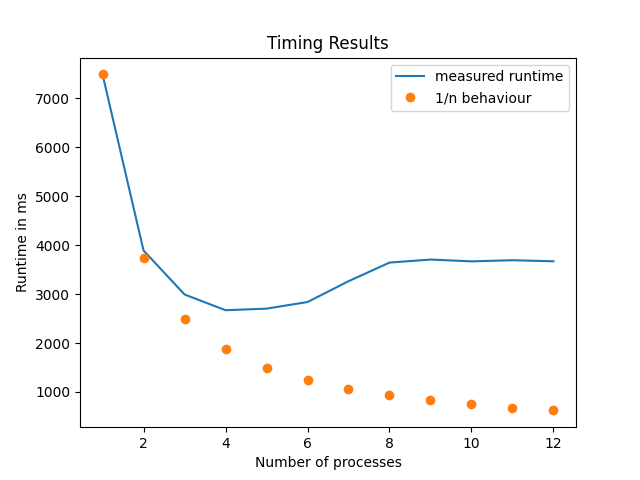
\includegraphics[width=\linewidth]{./gfx/09-cpu-count-1}
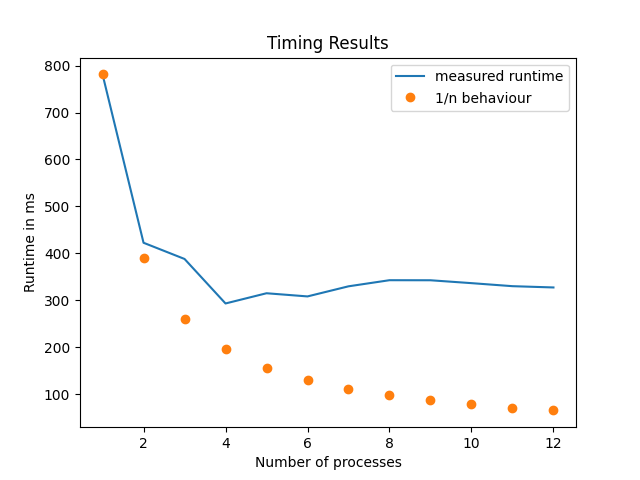
\includegraphics[width=\linewidth]{./gfx/09-cpu-count-2}
%
\column{.7\linewidth}
\begin{itemize}
\item Graphs: Solving the TSP on a machine with 4 logical processors + hyperthreading
	\begin{itemize}
	\item Orange dots: expectation (single thread runtime over number of processes)
	\item Blue: actual runtime
	\end{itemize}
\item Upper graph: hyperthreading does not live up to expectations on real world problems
\item Lower graph: even when only using logical processors, significant overhead
\item[\Thus] Optimal process number also depends whose machine you're using
	\begin{itemize}
	\item Your own: use all physical CPUs
	\item Your team's cluster: limit overhead!
	\end{itemize}
\end{itemize}
\end{columns}
%
\end{frame}
